\documentclass[manuscript,screen,nonacm]{acmart}
\setcopyright{none}
\settopmatter{printacmref=false,printccs=false}
\acmDOI{}\acmISBN{}
\usepackage{graphicx,xurl,placeins}
\setcitestyle{numbers}
\geometry{left=1in,right=1in,top=.75in,bottom=.65in,includeheadfoot}
\renewcommand{\topfraction}{.92}
\renewcommand{\bottomfraction}{.85}
\renewcommand{\textfraction}{.06}
\renewcommand{\floatpagefraction}{.80}
\setcounter{topnumber}{3}\setcounter{bottomnumber}{3}\setcounter{totalnumber}{5}
\setlength{\textfloatsep}{12pt plus 2pt minus 3pt}
\setlength{\intextsep}{12pt plus 2pt minus 3pt}
\raggedbottom
\title{Synthetic Creativity: Navigating Ordered Combinations of Disciplines}
\subtitle{Technical report; November 14, 2026.}
\author{William Taggart}
\affiliation{\department{Modern and Classical Languages and Literatures}\institution{Virginia Tech}\city{Blacksburg}\state{Virginia}\country{USA}}
\email{wtaggart@vt.edu}
\begin{document}
\begin{abstract}
Synthetic Creativity is a self-contained browser application for exploring interdisciplinary prompts through a two-dimensional matrix and a three-dimensional cube. Ordered pairs and triples of disciplines select deterministic role-based templates; cube rotation, cutaway depth, Z slices, and spreadsheet export offer complementary ways to inspect the combination space. The system uses no language-model service and makes no automatic judgment of novelty or value. This report develops its combinatorial model, interaction mapping, export structure, and limitations from the implementation.
\end{abstract}
\keywords{combinatorial creativity, interdisciplinary ideation, visual exploration, browser applications}
\maketitle
\section{Motivation and intellectual context}

An interdisciplinary idea can begin by assigning different roles to familiar fields: one supplies a method, another a problem domain, and a third a context or constraint. Synthetic Creativity makes this assignment explicit and repeatable. It offers candidate questions for interpretation rather than presenting generated combinations as validated discoveries.

Boden distinguishes different mechanisms of creativity, including the recombination of familiar ideas \cite{boden}. Creative Cognition examines the cognitive processes that can support invention and discovery \cite{finke}. Rhoten, O'Connor, and Hackett consider integrative creativity and collaborative disciplinary work \cite{rhoten}. These perspectives motivate structured encounters across domains, but none establishes that enumerating combinations alone produces creative achievement. The application's contribution is an inspectable interaction space; novelty, usefulness, feasibility, and disciplinary validity require subsequent judgment.

\begin{figure}[!htb]
% Balance the space above and below this figure and its caption.
\vspace*{8pt}
\centering
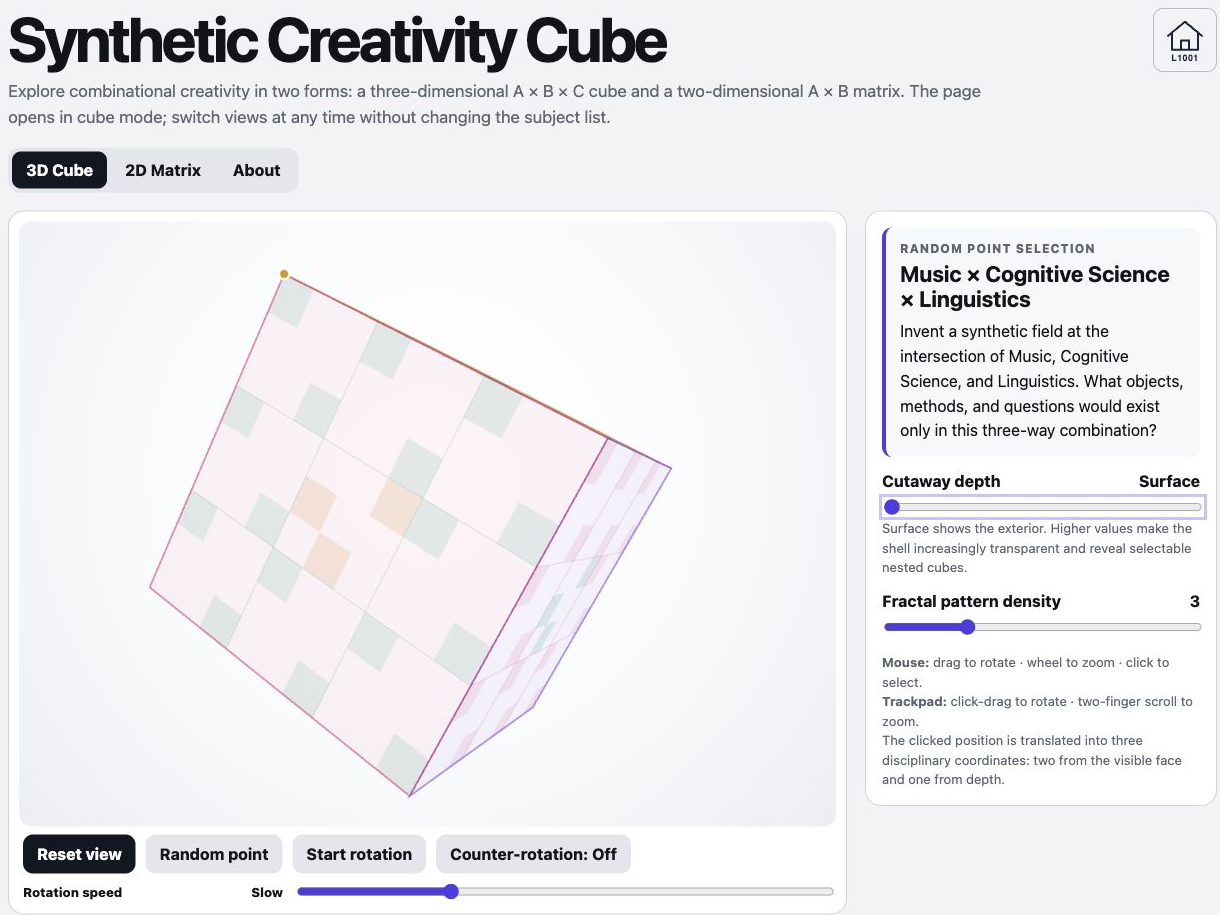
\includegraphics[width=.96\linewidth,height=.30\textheight,keepaspectratio]{figures/screenshot-01.png}
\caption{A selected ordered triple in the cube: Music, Cognitive Science, and Linguistics.}
\Description{A selected ordered triple in the cube: Music, Cognitive Science, and Linguistics.}
\label{fig:1}
\vspace*{-8pt}
\end{figure}

\section{Combinatorial model}

Let D be the ordered list of n subjects. The matrix indexes the Cartesian product D times D, and the cube indexes D times D times D. There are therefore n squared pair positions and n cubed triple positions, including combinations in which subjects repeat. With the default 50 disciplines, these counts are 2,500 and 125,000. They count ordered positions, not unique useful ideas.

Order matters because the templates assign roles. A field used as a method can yield a different question from the same field used as a domain or ethical complication. Repeated disciplines remain available as self-reflection rather than being removed as duplicates of cross-disciplinary combinations. A diagonal entry asks about a field's core inquiry instead of pretending that identical labels introduce independent expertise.

The displayed three-dimensional coordinates are indices in this combinatorial structure. They are not learned embeddings, estimates of similarity, emotional coordinates, or distances between disciplines. Adjacent positions primarily reflect the subject-list order. This limits any inference from visual proximity: two neighboring cells are not necessarily conceptually close.

\section{Deterministic prompt generation}

The pair generator selects one of five templates by adding row and column indices and taking the remainder modulo five. The triple generator uses the remainder of seven times the first index, eleven times the second, and thirteen times the third, again modulo five. Substitution inserts subject names into roles such as method, domain, context, audience, or constraint. Special cases handle identical subjects.

Given an unchanged list and indices, the prompt is reproducible without a network call. Reordering the subject list changes both the mapping of names to positions and the template selector. Thus reproducibility requires preserving the ordered list as well as the selected coordinates. The generator contains no language model, semantic retrieval, novelty filter, or learned ranking function. Its variability comes from position and template selection.

\begin{figure}[!htb]\vspace*{8pt}
\centering
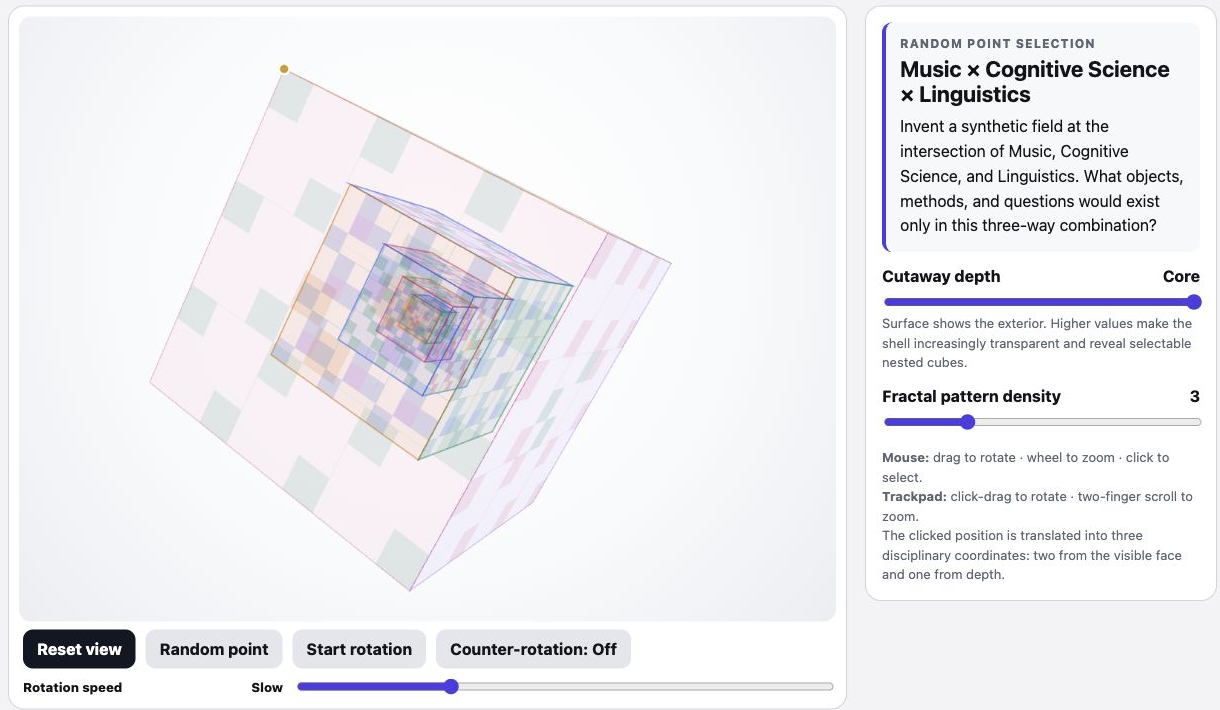
\includegraphics[width=.96\linewidth,height=.30\textheight,keepaspectratio]{figures/screenshot-02.png}
\caption{The core cutaway exposes nested cubes while retaining the selected disciplinary prompt.}
\Description{The core cutaway exposes nested cubes while retaining the selected disciplinary prompt.}
\label{fig:2}
\vspace*{-8pt}
\end{figure}

\section{Cube interaction and selection}

The browser draws the cube on a canvas. Users can rotate it by dragging, zoom, select a visible face, request a random point, start or pause rotation, and control counter-rotation. Face selection maps projected coordinates back to discrete indices; cutaway depth supplies the remaining layer. Index values are quantized and bounded to the valid subject range. Random selection chooses indices rather than searching for a particularly creative combination.

The cutaway display exposes nested cubes, with surface and core views and a density control. These nested structures support navigation and visual orientation. They do not increase the number of subject combinations beyond n cubed or add new inferred dimensions. The selected prompt appears alongside the visualization, so the user can read the role assignment independently of the rotating object.

\section{Editing subjects and inspecting slices}

Users enter one subject per line. The application trims lines and removes case-insensitive duplicates before rebuilding the matrix. Reset defaults restores the supplied disciplinary list. This permits smaller workshop-specific vocabularies or lists of methods, materials, and problems, although the built-in prompt wording still reflects the application's disciplinary framing. An empty or unsuitable vocabulary cannot be made meaningful by the cube representation alone.

\begin{figure}[!htb]\centering
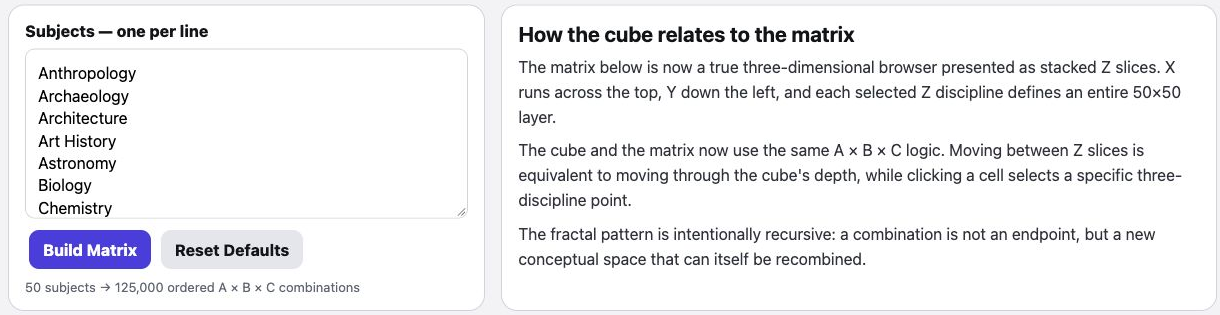
\includegraphics[width=.96\linewidth,height=.30\textheight,keepaspectratio]{figures/screenshot-03.png}
\caption{The editable discipline list and its relationship to the three-dimensional matrix.}
\Description{The editable discipline list and its relationship to the three-dimensional matrix.}
\label{fig:3}
\end{figure}

A Z slice fixes the third index and presents all n squared combinations of the remaining two indices as a table. Previous and next controls move through layers, and selecting a cell exposes its prompt. This is an alternative inspection surface for the same ordered triples, not a separate generative process. The cube emphasizes orientation and exploration, whereas the table permits systematic scanning and comparison.

\begin{figure}[!htb]\vspace*{4pt}
\centering
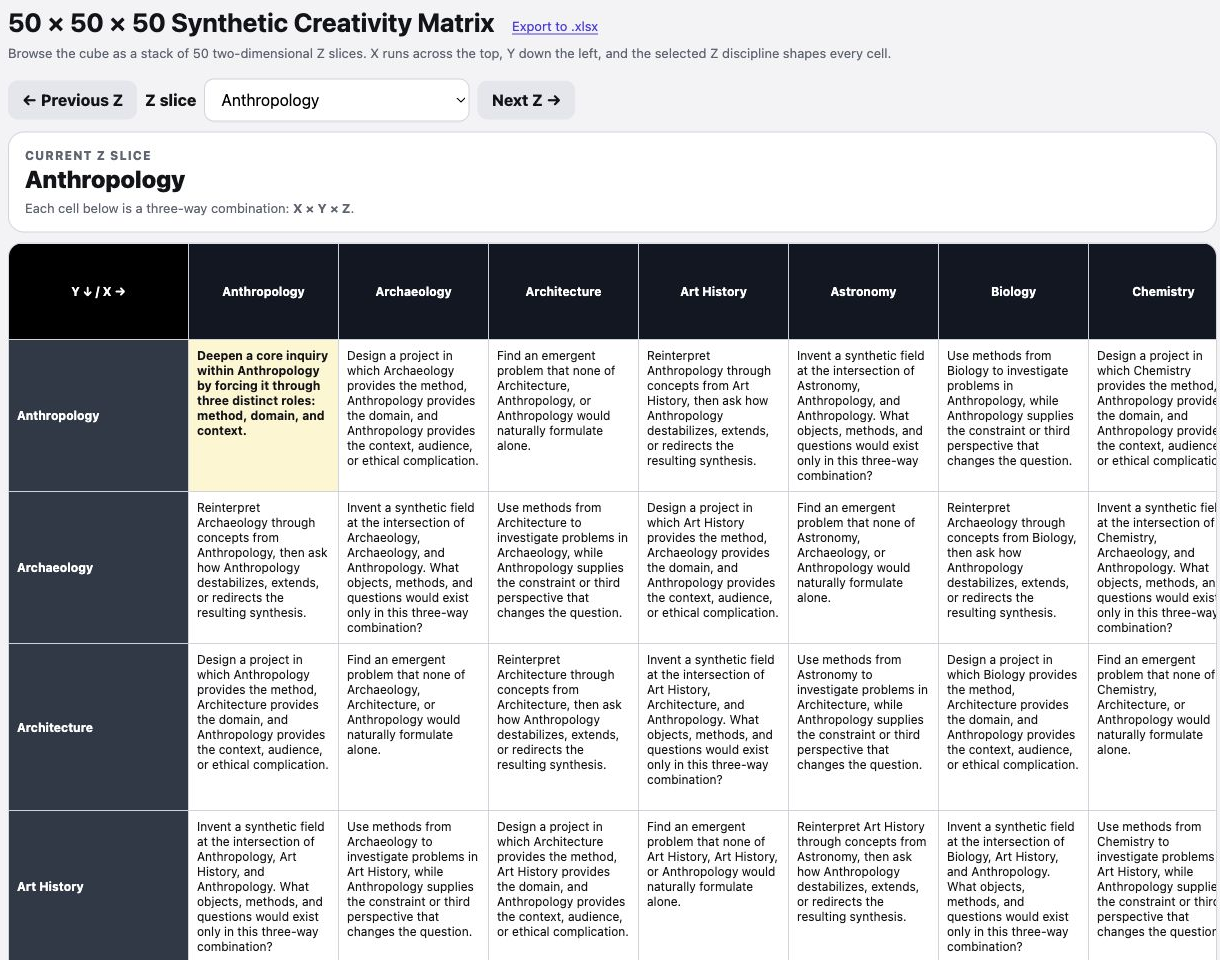
\includegraphics[width=.96\linewidth,height=.30\textheight,keepaspectratio]{figures/screenshot-04.png}
\caption{A Z-slice view exposes ordered triples as a two-dimensional table and offers spreadsheet export.}
\Description{A Z-slice view exposes ordered triples as a two-dimensional table and offers spreadsheet export.}
\label{fig:4}
\vspace*{-4pt}
\end{figure}

The separate two-dimensional mode operates on pairs. It has its own selected-cell question and matrix, and it uses the pair template rules rather than silently discarding the third role from a triple prompt. At the default list size, either table is already dense; zoom and viewport size affect legibility. Large custom lists therefore impose a practical usability limit even before computation becomes expensive.

\section{Spreadsheet export and computational costs}

The three-dimensional export generates an XLSX workbook with one worksheet per Z layer. Worksheet names are sanitized and constrained to the spreadsheet format's name length. Each sheet contains the corresponding grid of pair coordinates with the third subject fixed, making the full cube available outside the browser. The implementation creates the required workbook XML and ZIP container without a separate spreadsheet library.

\begin{figure}[!htb]\centering
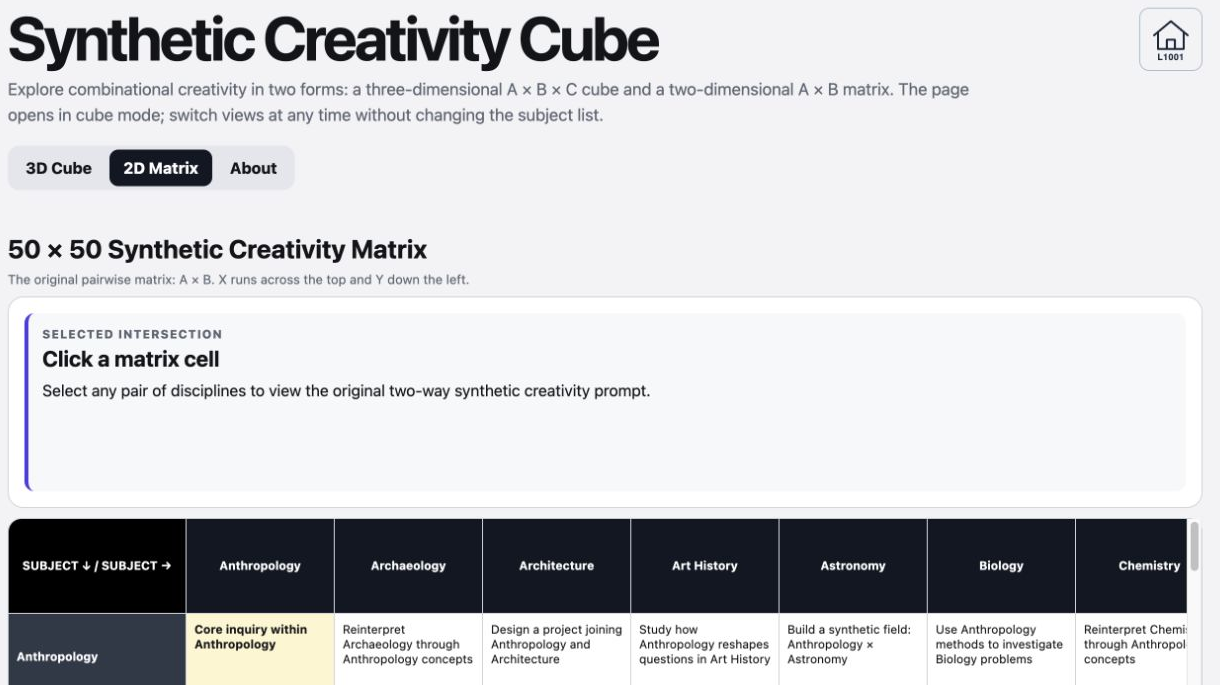
\includegraphics[width=.96\linewidth,height=.30\textheight,keepaspectratio]{figures/screenshot-05.png}
\caption{The separate two-dimensional matrix generates pairwise prompts rather than three-way prompts.}
\Description{The separate two-dimensional matrix generates pairwise prompts rather than three-way prompts.}
\label{fig:5}
\end{figure}

A visible slice needs work proportional to n squared, while full-cube export must enumerate n cubed prompts. Doubling the list length multiplies the conceptual cube and export workload by eight. These are asymptotic consequences of the implemented enumeration, not measured browser benchmarks. The application has no backend queue or external storage service to absorb that cost; large exports consume client memory and processing time.

Exported questions can support classroom exercises, research brainstorming, or collaborative selection. The workbook preserves generated prompts for review, but it does not document why a person judged one combination valuable. A rigorous ideation study would therefore need additional records of participant choices, subsequent refinement, and independent assessments of originality and usefulness.

\section{Deployment, evidence, and limitations}

The application consists of HTML, CSS, and JavaScript and can be opened in a modern browser without an API key, Python environment, or build step. The shown interface states were captured from the opened web application. They illustrate actual controls and deterministic prompts; they are not results from an experiment comparing creativity methods. No claim is made that the cube improves idea quality, reduces disciplinary bias, or produces publishable research proposals automatically.

Template repetition, the chosen vocabulary, list order, and users' prior knowledge strongly constrain the output. A prompt can combine names fluently while leaving methodological incompatibilities unresolved. The geometric display can also invite overinterpretation unless its index-based meaning remains clear. Future work could assess alternative templates, accessibility and keyboard navigation, vocabulary design, and expert ratings of selected prompts. Additional dimensions or model assistance are possible extensions, not features required by the present system.

\FloatBarrier
\section{AI disclosure}

This project was created with assistance from GPT-6 Astra and Codex. AI tools assisted with implementation and with drafting, checking, and formatting this report. William Taggart directed the project. This disclosure does not imply independent human validation of every generated statement; the implementation and cited sources remain available for review.


\bibliographystyle{ACM-Reference-Format}
\bibliography{references}
\end{document}
